%%
%% getstart.tex -- Flight Gear documentation: The FlightGear Manual
%% Chapter file
%%
%% Written by Michael Basler, started September 1998.
%%
%% Copyright (C) 2002 Michael Basler
%%
%%
%% This program is free software; you can redistribute it and/or
%% modify it under the terms of the GNU General Public License as
%% published by the Free Software Foundation; either version 2 of the
%% License, or (at your option) any later version.
%%
%% This program is distributed in the hope that it will be useful, but
%% WITHOUT ANY WARRANTY; without even the implied warranty of
%% MERCHANTABILITY or FITNESS FOR A PARTICULAR PURPOSE.  See the GNU
%% General Public License for more details.
%%
%% You should have received a copy of the GNU General Public License
%% along with this program; if not, write to the Free Software
%% Foundation, Inc., 675 Mass Ave, Cambridge, MA 02139, USA.
%%
%% $Id: flight.tex,v 0.5 0.6 2002/09/09 michael
%% (Log is kept at end of this file)

%%%%%%%%%%%%%%%%%%%%%%%%%%%%%%%%%%%%%%%%%%%%%%%%%%%%%%%%%%%%%%%%%%%%%%%%%%%%%%%%
%%%%%%%%%%%%%%%
\chapter{In-flight: All about instruments, keystrokes and menus\label{flight}}
%%%%%%%%%%%%%%%%%%%%%%%%%%%%%%%%%%%%%%%%%%%%%%%%%%%%%%%%%%%%%%%%%%%%%%%%%%%%%%%%
%%%%%%%%%%%%%%%
\markboth{\thechapter.\hspace*{1mm} FLIGHT}{\thesection\hspace*{1mm} KEYBOARD
CONTROLS}

The following is a description of the main systems for controlling the
program and piloting the plane: Historically, \Index{keyboard controls} were
developed
first, and you can still control most of the simulator via the keyboard alone.
Later on,
they were supplemented by several menu entries, making the interface more
accessible,
particularly for beginners, and providing additional functionality.

For getting a real feeling of flight, you should definitely consider
getting a \Index{joystick} or a \Index{yoke} plus
\Index{rudder pedals}. In any case, you can specify your device of
choice for control via the \texttt{-$ $-control-mode} option, i.e\.
select joystick, \Index{keyboard}, \Index{mouse}. The default setting
is joystick.

A short leaflet showing the standard keys can be found at
 \medskip

\web{http://www.flightgear.org/Docs/InstallGuide/FGShortRef.html}.
 \medskip

\noindent
A version of this leaflet can also be opened via \FlightGear{}'s help menu.

%%%%%%%%%%%%%%%%%%%%%%%%%%%%%%%%%%%%%%%%%%%%%%%%%%%%%%%%%%%%%%%%%%%%%%%%%%%%%%%%
%%%%%%%%%%%%%%%
\section{Starting the engine}\index{engine!starting}
%%%%%%%%%%%%%%%%%%%%%%%%%%%%%%%%%%%%%%%%%%%%%%%%%%%%%%%%%%%%%%%%%%%%%%%%%%%%%%%%
%%%%%%%%%%%%%%%

Depending on your situation, when you start the simulator the
\Index{engine}s may be on or off. When they are on you just can go on
with the start. When they are off, you have to start them first. The
\Index{ignition switch} for starting the engine is situated in the
lower left corner of the panel. It is shown in Fig.\,4.

\begin{figure}[!htp]
\centering
\includegraphics[width=0.5\textwidth]{magnet2}
\caption{The ignition switch.}
\end{figure}

It has five positions: ``OFF'', ``L'', ``R'', ``BOTH'', and ``START''.
The extreme right position is for starting the engine. For starting the
engine, put it onto the position ``BOTH'' using the mouse first.

Keep in mind that the \Index{mixture lever} has to be at 100\,\% (all
the way in) for starting the engine -- otherwise you will fail. In
addition, advance the \Index{throttle} to about 25\,\%.

Operate the \Index{starter} using the ``s'' key now. When pressing the
``s'' key you will observe the ignition switch to change to the
position ``START'' and the engine to start after a few seconds.
Afterwards you can bring the throttle back to idle (all the way out).

In addition, have a look if the \Index{parking brake}s are on (red
field lit). If so, press the ``B'' button to release them.

%%%%%%%%%%%%%%%%%%%%%%%%%%%%%%%%%%%%%%%%%%%%%%%%%%%%%%%%%%%%%%%%%%%%%%%%%%%%%%%%
%%%%%%%%%%%%%%%
\section{Keyboard controls}\index{keyboard controls}
%%%%%%%%%%%%%%%%%%%%%%%%%%%%%%%%%%%%%%%%%%%%%%%%%%%%%%%%%%%%%%%%%%%%%%%%%%%%%%%%
%%%%%%%%%%%%%%%

While \Index{joystick}s or \Index{yoke}s are supported as are \Index{rudder}
pedals, you can fly \FlightGear{} using the keyboard alone. For proper control
of the plane during flight via the keyboard (i) the \texttt{\Index{NumLock}}
key must be switched on (ii) the \FlightGear{} window must have focus (if not,
click with the mouse onto the graphics window). Several of the keyboard
controls might be helpful even if you use a joystick or yoke.

With the \texttt{NumLock} active, the following main \Index{keyboard controls}
for controlling the aircraft should work:
 \eject

\noindent
 Tab.\,2: \textit{Main \Index{keyboard controls} for \FlightGear{} on the
 numeric keypad with \texttt{NumLock} active.}
\medskip

\centerline{%%
%% tab2.tex -- Flight Gear documentation: The FlightGear Manual
%% Keyboard controls table 1/Main controls
%%
%% Written by Michael Basler, started September 1998.
%%
%% Copyright (C) 2002 Michael Basler
%%
%%
%% This program is free software; you can redistribute it and/or
%% modify it under the terms of the GNU General Public License as
%% published by the Free Software Foundation; either version 2 of the
%% License, or (at your option) any later version.
%%
%% This program is distributed in the hope that it will be useful, but
%% WITHOUT ANY WARRANTY; without even the implied warranty of
%% MERCHANTABILITY or FITNESS FOR A PARTICULAR PURPOSE.  See the GNU
%% General Public License for more details.
%%
%% You should have received a copy of the GNU General Public License
%% along with this program; if not, write to the Free Software
%% Foundation, Inc., 675 Mass Ave, Cambridge, MA 02139, USA.
%%
%% $Id: tab1.tex,v 0.6 2002/09/09 michael
%% (Log is kept at end of this file)
%%%%%%%%%%%%%%%%%%%%%%%%%%%%%%%%%%%%%%%%%%%%%%%%%%%%%%%%%%%%%%%%%%%%%%%%%%%%%%%%%%%%%%%%%%%%%%%%
\begin{tabular}{|l|l|}\hline
\IfLanguageName{english}{
  Key      &  Action\\\hline
 9 / 3     &  Throttle\index{throttle}\\
 4 / 6     &  Aileron\index{aileron}\\
 8 / 2     &  Elevator\index{elevator}\\
 0 / Enter &  Rudder\index{rudder}\\
 5         &  Center aileron/elevator/rudder\\
 7 / 1     &  Elevator \Index{trim}\\\hline
}{}
\IfLanguageName{french}{
  Touche      &  Action\\\hline
 9 / 3     &  Commande des gaz\index{gaz}\\
 4 / 6     &  Aileron\index{aileron}\\
 8 / 2     &  Gouverne de profondeur\index{gouverne de profondeur}\\
 0 / Entr\'{e}e &  gouverne de direction\index{gouverne de direction}\\
 5         &  Centrage des ailerons/gouverne de profondeur/direction\\
 7 / 1     &  Trim de la gouverne de profondeur \Index{trim}\\\hline
}{}
\IfLanguageName{italian}{
  Pulsante/i      &  Azione\\\hline
 9 / 3     &  Manetta (Throttle)\index{manetta}\index{throttle}\\
 4 / 6     &  Alettoni\index{Alettoni}\\
 8 / 2     &  Elevatore (timone di coda)\index{Elevatore}\\
 0 / Invio &  Timone di direzione\index{gouverne de direction}\\
 5         &  Centra alettoni, timone di coda e di direzione\\
 7 / 1     &  Regola il trim \Index{trim}\\\hline
}{}

\end{tabular}

%% revision 0.5 2002/02/15 michael
%% Initial revision
}
%%% \noalign{\vskip 5mm}
\vskip 5mm

For changing views you have to de-activate \texttt{NumLock}. Now \texttt{Shift}
+
$<$\texttt{Numeric Keypad Key}$>$ changes the view as follows:
\medskip

\noindent
 Tab.\,3: \textit{View directions\index{view directions}
accessible after de-activating \texttt{NumLock} on the numeric keypad.}
\medskip

\centerline{%%
%% tab3.tex -- Flight Gear documentation: The FlightGear Manual
%% Keyboard controls table 2/View directions
%%
%% Written by Michael Basler, started September 1998.
%%
%% Copyright (C) 2002 Michael Basler
%%
%%
%% This program is free software; you can redistribute it and/or
%% modify it under the terms of the GNU General Public License as
%% published by the Free Software Foundation; either version 2 of the
%% License, or (at your option) any later version.
%%
%% This program is distributed in the hope that it will be useful, but
%% WITHOUT ANY WARRANTY; without even the implied warranty of
%% MERCHANTABILITY or FITNESS FOR A PARTICULAR PURPOSE.  See the GNU
%% General Public License for more details.
%%
%% You should have received a copy of the GNU General Public License
%% along with this program; if not, write to the Free Software
%% Foundation, Inc., 675 Mass Ave, Cambridge, MA 02139, USA.
%%
%% $Id: tab2.tex,v 0.6 2002/09/09 michael
%% (Log is kept at end of this file)
%%%%%%%%%%%%%%%%%%%%%%%%%%%%%%%%%%%%%%%%%%%%%%%%%%%%%%%%%%%%%%%%%%%%%%%%%%%%%%%%%%%%%%%%%%%%%%%%
\begin{tabular}{|c|l|}\hline
\iflanguage{english}{
   Numpad Key  &  View direction\index{view directions}\\\hline
    Shift-8  & Forward\\
    Shift-7  & Left/forward\\
    Shift-4  & Left\\
    Shift-1  & Left/back\\
    Shift-2  & Back\\
    Shift-3  & Right/back\\
    Shift-6  & Right\\
    Shift-9  & Right/forward\\\hline
}{}
\iflanguage{french}{
   Touche pav\'{e} num\'{e}rique & Angle de vue\index{angle de vue}\\\hline
    Shift-8  & Vers l'avant\\
    Shift-7  & Avant/Gauche\\
    Shift-4  & Gauche\\
    Shift-1  & Arri\`{e}re/Gauche\\
    Shift-2  & Arri\`{e}re\\
    Shift-3  & Arri\`{e}re/Droit\\
    Shift-6  & Droit\\
    Shift-9  & Avant/Droit\\\hline
}{}
\end{tabular}

%% revision 0.5 2002/02/15 michael
%% Initial revision
}
%%% \noalign{\vskip 5mm}
\vskip 5mm
Besides, there are several more options for adapting display on screen:
\vfill
\eject

\noindent
 Tab.\,4: \textit{Display options\index{display options}}
\medskip

\centerline{%%
%% tab4.tex -- Flight Gear documentation: Installation and Getting Started
%% Keyboard controls table 3/Additional view options
%%
%% Written by Michael Basler, started September 1998.
%%
%% Copyright (C) 2002 Michael Basler (pmb@epost.de)
%%
%%
%% This program is free software; you can redistribute it and/or
%% modify it under the terms of the GNU General Public License as
%% published by the Free Software Foundation; either version 2 of the
%% License, or (at your option) any later version.
%%
%% This program is distributed in the hope that it will be useful, but
%% WITHOUT ANY WARRANTY; without even the implied warranty of
%% MERCHANTABILITY or FITNESS FOR A PARTICULAR PURPOSE.  See the GNU
%% General Public License for more details.
%%
%% You should have received a copy of the GNU General Public License
%% along with this program; if not, write to the Free Software
%% Foundation, Inc., 675 Mass Ave, Cambridge, MA 02139, USA.
%%
%% $Id: tab3.tex,v 0.6 2002/09/09 michael
%% (Log is kept at end of this file)
%%%%%%%%%%%%%%%%%%%%%%%%%%%%%%%%%%%%%%%%%%%%%%%%%%%%%%%%%%%%%%%%%%%%%%%%%%%%%%%%%%%%%%%%%%%%%%%%
\begin{tabular}{|l|l|}\hline
 Key              &         Action\\\hline
 P                &    Toggle \Index{instrument panel} on/off \\
 c                &    Toggle3D/2D cockpit
 											 \index{2D cockpit} (if both are available)
 											 \index{3D cockpit}\index{cockpit}\\
 s                &    Cycle panel style full/mini\\
 Shift-F5/F6      &    Shift the panel in y direction\\
 Shift-F7/F8      &    Shift the panel in x direction\\
 Shift-F3					&    Read a panel from a property list\\
 i/I              &    Minimize/maximize HUD              \\
 h/H              &    Change color  of HUD/toggle HUD off\\
                  &    forward/backward      \\   \hline
  x/X             &    Zoom in/out\\
   v              &    Cycle \Index{view modes} (pilot, chase, tower)\\ \hline
   W              &    Toggle \Index{full screen mode} on/off (3dfx only)\\
   z/Z            &    Change \Index{visibility} (fog)  forward/backward \\
   F8             &    Toggle fog on/off\\
   F2			 				& 	 Refresh Scenery tile cache\\
   F4			 				& 	 Force Lighting update\\
   F9             &    Toggle texturing on/off\\
   F10      			&    Toggle menu on/off\\ \hline   
 \end{tabular}

%% revision 0.5 2002/02/15 michael
%% Initial revision}
%%% \noalign{\vskip 5mm}
\vskip 5mm

The \Index{autopilot} is controlled via the following keys:
\medskip

\noindent
 Tab.\,5: \textit{Autopilot and related controls.\index{autopilot controls}}
\medskip

\centerline{%%
%% tab5.tex -- Flight Gear documentation: Installation and Getting Started
%% Keyboard controls table 4/autopilot controls
%%
%% Written by Michael Basler, started September 1998.
%%
%% Copyright (C) 2002 Michael Basler
%%
%%
%% This program is free software; you can redistribute it and/or
%% modify it under the terms of the GNU General Public License as
%% published by the Free Software Foundation; either version 2 of the
%% License, or (at your option) any later version.
%%
%% This program is distributed in the hope that it will be useful, but
%% WITHOUT ANY WARRANTY; without even the implied warranty of
%% MERCHANTABILITY or FITNESS FOR A PARTICULAR PURPOSE.  See the GNU
%% General Public License for more details.
%%
%% You should have received a copy of the GNU General Public License
%% along with this program; if not, write to the Free Software
%% Foundation, Inc., 675 Mass Ave, Cambridge, MA 02139, USA.
%%
%% $Id: tab4.tex,v 0.6 2002/09/09 michael
%% (Log is kept at end of this file)
%%%%%%%%%%%%%%%%%%%%%%%%%%%%%%%%%%%%%%%%%%%%%%%%%%%%%%%%%%%%%%%%%%%%%%%%%%%%%%%%%%%%%%%%%%%%%%%%
\begin{tabular}{|l|l|}\hline
 Key              &         Action\\\hline
    Ctrl + A      &         Altitude hold\index{altitude hold} toggle on/off\\
    Ctrl + G      &         Follow glide slope 1 toggle on/off\\
    Ctrl + H      &         Heading hold\index{heading hold} toggle on/off\\
    Ctrl + N      &         Follow NAV 1 radial toggle on/off\\
    Ctrl + S      &         Autothrottle\index{autothrottle} toggle on/off\\
    Ctrl + T      &         Terrain follow toggle on/off\\
    Ctrl + U      &         Add 1000 ft. to your altitude (emergency)\\
    Enter		      &         Increase autopilot heading\\
    F6 		    		&         Toggle autopilot target:\\
                  &         current heading/waypoint\\
    F11           &         Autopilot altitude dialog\\
    F12           &         Autopilot heading dialog\\\hline
\end{tabular}

%% revision 0.5 2002/02/15 michael
%% Initial revision}
\medskip

\noindent Ctrl + T is especially interesting as it makes your little Cessna
behave
like a cruise missile. Ctrl + U might be handy in case you feel you're just
about to
crash. (Shouldn't real planes sport such a key, too?)

In case the \Index{autopilot} is enabled, some of the numeric keypad keys get a
special
meaning:

\noindent
 Tab.\,6: \textit{Special action of keys, if autopilot is
 enabled.\index{autopilot controls} [U.S. keyboard uses "." instead of ","]}
\medskip

\centerline{%%
%% tab6.tex -- Flight Gear documentation: Installation and Getting Started
%% Keyboard controls table 5/key actions for autopilot enabled
%%
%% Written by Michael Basler, started September 1998.
%%
%% Copyright (C) 2002 Michael Basler (pmb@epost.de)
%%
%%
%% This program is free software; you can redistribute it and/or
%% modify it under the terms of the GNU General Public License as
%% published by the Free Software Foundation; either version 2 of the
%% License, or (at your option) any later version.
%%
%% This program is distributed in the hope that it will be useful, but
%% WITHOUT ANY WARRANTY; without even the implied warranty of
%% MERCHANTABILITY or FITNESS FOR A PARTICULAR PURPOSE.  See the GNU
%% General Public License for more details.
%%
%% You should have received a copy of the GNU General Public License
%% along with this program; if not, write to the Free Software
%% Foundation, Inc., 675 Mass Ave, Cambridge, MA 02139, USA.
%%
%% $Id: tab5.tex,v 0.6 2002/09/09 michael
%% (Log is kept at end of this file)
%%%%%%%%%%%%%%%%%%%%%%%%%%%%%%%%%%%%%%%%%%%%%%%%%%%%%%%%%%%%%%%%%%%%%%%%%%%%%%%%%%%%%%%%%%%%%%%%
\begin{tabular}{|l|l|}\hline
 Key           &         Action\\\hline
    8 / 2      &         Altitude adjust\\
    0 / ,      &         Heading adjust\\
    9 / 3      &         Autothrottle adjust \\\hline
 \end{tabular}

%% revision 0.5 2002/02/15 michael
%% Initial revision}
\medskip

There are several keys for starting and controlling the engine \index{engine
controls}:

\noindent
 Tab.\,7: \textit{Engine control keys}
\medskip

\centerline{%%
%% tab7.tex -- Flight Gear documentation: The FlightGear Manual
%% Keyboard controls table 6/Engine related controls
%%
%% Written by Michael Basler, started September 1998.
%%
%% Copyright (C) 2002 Michael Basler
%%
%%
%% This program is free software; you can redistribute it and/or
%% modify it under the terms of the GNU General Public License as
%% published by the Free Software Foundation; either version 2 of the
%% License, or (at your option) any later version.
%%
%% This program is distributed in the hope that it will be useful, but
%% WITHOUT ANY WARRANTY; without even the implied warranty of
%% MERCHANTABILITY or FITNESS FOR A PARTICULAR PURPOSE.  See the GNU
%% General Public License for more details.
%%
%% You should have received a copy of the GNU General Public License
%% along with this program; if not, write to the Free Software
%% Foundation, Inc., 675 Mass Ave, Cambridge, MA 02139, USA.
%%
%% $Id: tab6.tex,v 0.6 2002/09/09 michael
%% (Log is kept at end of this file)
%%%%%%%%%%%%%%%%%%%%%%%%%%%%%%%%%%%%%%%%%%%%%%%%%%%%%%%%%%%%%%%%%%%%%%%%%%%%%%%%%%%%%%%%%%%%%%%%
\begin{tabular}{|l|l|}\hline
  \ifchinese
  按键   &    操作\\\hline
  !     &    选择第一号发动机\\
  @     &    选择第二号发动机\\
  \#    &    选择第三号发动机\\
  \$    &    选择第四号发动机\\
  $\sim$$ &  选择所有发动机\\\hline
  \{    &    减少所选发动机的磁电机档位\\
  \}    &    增加所选发动机的磁电机档位\\
  s     &    为所选的发动机点火启动\\
  M / m &    贫油/富油所选发动机的油气混合比\\
  N / n &    减少/增加所选发动机的螺旋桨转速 \\\hline
  \fi
\iffalse
\IfLanguageName{english}{
Key      &  Action\\ \hline
   !     & Select 1st engine\\
   @	   & Select 2nd engine\\
  \#     & Select 3rd engine\\
  \$     & Select 4th engine\\
  $\sim$ & Select all engines\\\hline
  \{     & Decrease magneto on selected engine\\
  \}     & Increase magneto on selected engine\\
   s     & Fire starter on selected engine(s)\\
  M / m  & Lean/Enrich selected engine mixture\\
  N / n  & Decrease/Increase selected propeller RPM\\\hline
}{}
\fi
\IfLanguageName{french}{
Touche     &  Action\\ \hline
   !     & S\'{e}l\'{e}ctionne le premier moteur\\
   @	 & S\'{e}l\'{e}ctionne le deuxi\`{e}me moteur\\
  \#     & S\'{e}l\'{e}ctionne le troisi\`{e}me moteur\\
  \$     & S\'{e}l\'{e}ctionne le quatri\`{e}me moteur\\
  $\sim$ & S\'{e}l\'{e}ctionne tous les moteurs\\\hline
  \{     & D\'{e}cr\'{e}mente le magn\'{e}to sur le moteur s\'{e}lectionn\'{e}\\
  \}     & Incr\'{e}mente le magn\'{e}to sur le moteur s\'{e}lectionn\'{e}\\
   s     & D\'{e}marrage du/des moteur(s) s\'{e}lectionn\'{e}(s)\\
  M / m  & Appauvrir/Enrichir le m\'{e}lange du moteur s\'{e}lectionn\'{e}\\
  N / n  & Diminue/Augmente le nombre de tours par minute du moteur s\'{e}lectionn\'{e}\\\hline
}{}
\IfLanguageName{italian}{
Pulsante/i &  Azione\\ \hline
   !     & Seleziona il 1\textdegree{} motore\\
   @	   & Seleziona il 2\textdegree{} motore\\
  \#     & Seleziona il 3\textdegree{} motore\\
  \$     & Seleziona il 4\textdegree{} motore\\
  $\sim$ & Seleziona tutti i motori\\\hline
  \{     & Diminuisce la forza dei magneti sui motori selezionati\\
  \}     & Aumenta la forza dei magneti sui motori selezionati\\
   s     & Avvia i(l) motore/i selezionato/i\\
  M / m  & Impoverisce/Arricchisce la miscela del motore selezionato\\
  N / n  & Diminuisce/Aumenta il passo dell'elica del motore selezionato\\\hline
}{}
\end{tabular}

%% revision 0.5 2002/02/15 michael
%% Initial revision
}
\medskip

Beside these basic keys there are miscellaneous keys for special
actions; some of these you'll probably not want to try during your
first flight:
\vfill
\eject

\noindent Tab.\,8: \textit{Miscellaneous keyboard controls.\index{keyboard
controls! miscellaneous}}
\medskip

\centerline{%%
%% tab8.tex -- Flight Gear documentation: The FlightGear Manual
%% Keyboard controls table 7/Miscellaneous
%%
%% Written by Michael Basler, started September 1998.
%%
%% Copyright (C) 2002 Michael Basler
%%
%%
%% This program is free software; you can redistribute it and/or
%% modify it under the terms of the GNU General Public License as
%% published by the Free Software Foundation; either version 2 of the
%% License, or (at your option) any later version.
%%
%% This program is distributed in the hope that it will be useful, but
%% WITHOUT ANY WARRANTY; without even the implied warranty of
%% MERCHANTABILITY or FITNESS FOR A PARTICULAR PURPOSE.  See the GNU
%% General Public License for more details.
%%
%% You should have received a copy of the GNU General Public License
%% along with this program; if not, write to the Free Software
%% Foundation, Inc., 675 Mass Ave, Cambridge, MA 02139, USA.
%%
%% $Id: tab7.tex,v 0.5 2002/15/02 michael
%% (Log is kept at end of this file)
%%%%%%%%%%%%%%%%%%%%%%%%%%%%%%%%%%%%%%%%%%%%%%%%%%%%%%%%%%%%%%%%%%%%%%%%%%%%%%%%%%%%%%%%%%%%%%%%
\begin{tabular}{|l|l|}\hline
  \ifchinese
  按键       &    操作\\\hline
  b         &    启用所有\Index{刹车}\\
  , / .     &    启用左右刹车\\
            &    (用于\Index{差动刹车})\\
  l         &    切换\Index{尾轮锁定}\\
  B         &    切换停留刹车 \index{刹车}\index{停留刹车}\\
  g / G     &    收起/放下起落架 \index{机轮}\index{起落架}\\
  空格       &    按键通话(PTT)\\
  - / \_    &    多人飞行时文字聊天菜单/输入\\
  $[$ / $]$ &    收起/放下\Index{襟翼}\\
  j / k     &    收起/张开\Index{扰流板}\\
  CTRL-B    &    切换\Index{减速板}\\\hline
  \fi
\iffalse
\IfLanguageName{english}{
Key           &  Action\\\hline
  b           & Apply  all \Index{brakes}\\
  , / .       & Apply left/right brake \\
              & (useful for \Index{differential braking})\\
  l           & Toggle \Index{tail-wheel lock}\\
  B           & Toggle parking brake \index{brakes}\index{parking brake}\\
  g/G         & Raise/lower landing gear\index{gear}\index{landing gear}\\
  Space       & Push To Talk (PTT)\\
  - / \_      & MP text chat menu/entry\\
  $[$ / $]$   & Retract/extend \Index{flaps}\\
  j / k       & Retract/extend \Index{spoilers}\\
  Ctrl-B      & Toggle \Index{speed brakes}\\ \hline
}{}
\fi
\IfLanguageName{french}{
Touche        &  Action\\\hline
  b           & Appliquer tous les \Index{freins}\\
  , / .       & Appliquer le frein gauche/droit\\
              & (utile pour le \Index{freinage diff\'{e}rentiel})\\
  l           & Active le \Index{verrouillage de la roue de queue}\\
  B           & Active le frein de parking \index{freins}\index{freins de parking}\\
  g/G         & Monter/descendre le train d'atterrissage\index{train d'atterrissage}\index{train d'atterrissage}\\
  Espace      & Appuyez pour parler (Push To Talk, PTT)\\
  - / \_      & Entr\'{e}e/menu du clavardage clavier du mode multijoueurs\\
  $[$ / $]$   & Rentre/d\'{e}ploie les \Index{volets}\\
  j / k       & Rentre/d\'{e}ploie les \Index{a\'{e}rofreins}\\
  Ctrl-B      & Active les \Index{freins de vitesse}\\ \hline
}{}
\IfLanguageName{italian}{
Pulsante/i     &  Azione\\\hline
  b           & Applica tutti i \Index{freni} (tenere premuto)\\
  , / .       & Applica/Toglie il freno di sinistra/destra \\
  l           & Mette/Toglie il \Index{blocco delle ruote di coda}\\
  B           & Toglie/Mette i \Index{freni di parcheggio}\\
  g/G         & Alza/Abbassa il carrello d'atterraggio\index{carrello d'atterraggio}\\
  Space       & Tenendolo premuto si parla usando FGCom (PTT)\\
  - / \_      & Comandano la chat scritta\\
  $[$ / $]$   & Ritrae/Estende i \Index{flaps}\\
  j / k       & Ritrae/Estende i \Index{deflettori}\\
  Ctrl-B      & Applica/Toglie gli \Index{aerofreni}\\ \hline
}{}
\end{tabular}

%% revision 0.5 2002/02/15 michael
%% Initial revision
}
\medskip

\noindent
 Note: If you have difficulty processing the \Index{screenshot}
\texttt{fgfs-screen.ppm}
on a windows machine, just recall that simply pressing the ``Print'' key copies
the
screen to the clipboard, from which you can paste it into any graphics program.

These key bindings\index{keybindings!configuration} are not hard coded, but
user-adjustable.
You can check and change these setting via the file
\texttt{keyboard.xml}\index{keyboard.xml} to be found in the main
\FlightGear{} directory. This is a human readable plain ASCII file.
Although it's perhaps not the best idea for beginners to start just
with modifying this file, more advanced users will find it useful to
change key bindings according to what they like (or, perhaps, know from
other simulators).

%%%%%%%%%%%%%%%%%%%%%%%%%%%%%%%%%%%%%%%%%%%%%%%%%%%%%%%%%%%%%%%%%%%%%%%%%%%%%%%%
%%%%%%%%%%%%%%%
\section{Menu entries}\index{menu entries}
%%%%%%%%%%%%%%%%%%%%%%%%%%%%%%%%%%%%%%%%%%%%%%%%%%%%%%%%%%%%%%%%%%%%%%%%%%%%%%%%
%%%%%%%%%%%%%%%

If you want to hide the menu after applying some changes, just hit F10.

The menu provides the following sub-menus and options.

\begin{itemize}
 \item \textbf{File}
 \begin{itemize}
  \item \textbf{Save flight} Saves\index{save flight} the current flight, by
default to \texttt{fgfs.sav}.
 \item \textbf{Load flight} Loads\index{load flight} the current flight, by
default from \texttt{fgfs.sav}. You should
start \FlightGear{} using the same options (aircraft, airport...) as when you
saved the flight.
 \item \textbf{Reset} Resets\index{reset flight} you to the selected starting
position.
 Comes handy in case you got lost or something went wrong.
  \item \textbf{High-Res Snap Shot} Saves a high resolution screen
shot\index{screenshot} as \\ \texttt{fgfs-screen-XXX.ppm} under
  the directory you started the program from.
  \item \textbf{Snap Shot} Saves a normal resolution screen
shot\index{screenshot} as \\ \texttt{fgfs-screen-XXX.ppm} under
  the directory you started the program from.
  \item \textbf{Print Screen} Prints screen shot (Linux only).
  \item \textbf{Sound Configuration} Allows you to mute sound, set the volume
and enable/disable ATC Chatter.
  ATC Chatter plays a number of real-life ATC communications to add realism.
  \item \textbf{Browse Internal Properties} Displays a tree view of all the
properties within the system.
  You can navigate through the tree like a graphical directory listing and set
properties by clicking on them
  \item \textbf{Logging} Allows you to log various pieces of flight information
to a file.
  You can set the file to log to, the properties to be logged and the interval
between logs.
  \item \textbf{Quit} Exits\index{exit} the program.
 \end{itemize}

 \item \textbf{View}\index{view}
 \begin{itemize}
  \item \textbf{Toggle 2D Panel}  Switches between a 2D panel and a 3D cockpit
(if available).
  \item \textbf{Toggle Dynamic Cockpit View}  Toggle between a fixed view-point
  (controlled by the mouse) and one that simulates the movement of your head as
  you fly the aircraft.
  \item \textbf{Rendering Options} Displays a dialog allowing you to toggle
various advanced graphical options.
  This allows you to trade eye-candy such as shadows, 3D clouds and specular
reflections for frame-rate.
  To help you achieve a good balance, enable the "Show Frame Rate" option.
  This displays the current frame-rate in frames-per-second in the bottom right
of the screen.
  Most people find a frame-rate of around 20fps adequate for flying. The
frame-rate is affected by the
  graphical options you have enabled, the current visibility (set by Z/z), the
number of objects in view
  and their level of detail (LOD).
  \item \textbf{G-force Options}  Displays a dialog allowing you to configure
how your bodies reaction to G-forces is simulated. This includes black-out due
to high G, and redout due to negative G.
  \item \textbf{Adjust View Distance}  Displays a dialog showing the current
view offset.
  You can adjust this by dragging the dials. Alternatively you can make small
adjustments
  to your view-point using the mouse (see below).
  \item \textbf{Adjust HUD Properties}  Displays a dialog allowing you to set
the HUD settings, such as transparency and whether anti-aliasing is used to display it.
  \item \textbf{Instant Replay} Displays a dialog to control the instant replay
feature.
  A good tool for checking your landings! Press ``p'' to end the replay and
pause the flight.
  \item \textbf{Adjust LOD Ranges} Displays a dialog allowing you to set the
range at which different
  levels of detail are displayed. This affects the textures and objects
displayed in the simulator.
  \item \textbf{Chat} Displays a dialog allowing you chat with other aircraft in
the multi-player environment.
  \item \textbf{Chat Menu} Displays a menu of chat messages which you can
  transmit to other aircraft in the multi-player environment. Some menus
  contain sub-menus of options.
 \end{itemize}

\item \textbf{Location}\index{location}
 \begin{itemize}
   \item \textbf{Position Aircraft (on ground)}  Displays a dialog allowing you
to position the aircraft
   on the runway of any installed airport. You need to know the ICAO code for
the airport you wish to
   start from (e.g. KSFO for San Fransisco International).
   \item \textbf{Position Aircraft (in air)} Displays a dialog allowing you to
position the aircraft at
   an arbitary point in the air. You must select a known ground point, e.g. an
airport, VOR, long/lat
   coordinates, and a position relative to that point, e.g distance, direction,
altitude. You can also
   set your initial speed and heading. This is useful for practising approaches.
   \item \textbf{Select Airport from List} This allows you to select an airport
without knowing its ICAO
   code. You can search amongst all the airports that you have installed.
Clicking Apply will place you at that airport on a runway appropriate for the current wind.
   \item \textbf{Random Attitude} Sets the aircraft with a random heading, speed
and attitude. Useful for practising recovery from unusual attitudes.
   \item \textbf{Tower position} Displays a dialog allowing you to change the
airport tower used for the Tower View and Tower View Look From.
 \end{itemize}

\item \textbf{Autopilot}\index{autopilot} This menu is only available for
aircraft that have the default
autopilot configured. Other aircraft may have their own autopilot which is
configured through the panel.
 \begin{itemize}

   \item \textbf{Autopilot Settings} Displays a dialog allowing you to set the
aircraft autopilot.
   You can set the autopilot up in a variety of different ways - from simply
keeping the wings level, to following an ILS.
  \item \textbf{Route Manager} Edit the route (waypoint) list for the autopilot.
Waypoints can be airports or fixes. The heading, distance and time to the
current waypoint is displayed in the HUD.
  \item \textbf{Pop Waypoint} Pops the top waypoint from the route list.
 \item \textbf{Clear Route} Clears current route.
  \item \textbf{Set Lat/Lon Format} Toggles the HUD Latitude/Longitude format
between decimal minutes and seconds.
 \end{itemize}

\item \textbf{Environment}\index{weather}
 \begin{itemize}
  \item \textbf{Weather Scenario} Displays a dialog showing the current weather
reported by the closest
  weather station (usually an airport) as a METAR. You can change the weather
scenario between
  Fair Weather (clear skies, few clouds, little wind), a Thunderstorm (clouds,
rain, lightning), the current METAR, or none.
  \item \textbf{Weather Conditions}  Displays a dialog allowing you to set the
wind direction, wind speed,
  turbulence, visibility, temperature, dew point, barometer setting at various
altitudes.
  \item \textbf{Clouds}  Displays a dialog allowing you to set the cloud types,
elevations and thicknesses.
  Note that this affects 2D clouds only. 3D clouds (if enabled) are configured
through the Rendering Options menu.
  \item \textbf{Time Settings}  Displays a dialog allowing you to set the current
time in the simulator, speed up the simulation, and change the rate at which
time passes in the simulator. Also displays UTC and local time.
  \item \textbf{Rain/Snow Settings}  Displays a dialog allowing you to
configure how rain and snow is displayed.
 \end{itemize}

\item \textbf{Equipment}\index{equipment}
 \begin{itemize}
  \item \textbf{Fuel and Payload}  For aircraft that support it, allows you to
set the fuel and levels
  and current payload within the aircraft.
  \item \textbf{Radio Settings}  Displays a dialog allowing you to set the
frequencies and radials being
  used by the radios and navigational equipment.
  \item \textbf{GPS Settings}  Displays a dialog allowing you to set waypoints
and view course information for the GPS.
  \item \textbf{Instrument Settings}  Displays a dialog allowing you to set the
altimeter pressure and Heading Indicator offset.
  \item \textbf{System Failures} Displays a dialog allowing you to fail various
aircraft systems, such as the vacuum.
  \item \textbf{Instrument Failures}  Displays a dialog allowing you to fail
specific aircraft instruments.
 \end{itemize}

\item \textbf{ATC/AI}\index{ATC}\index{AI}
 \begin{itemize}
  \item \textbf{Frequencies}  Displays a dialog allowing you enter the ICAO code
for an airport
  (or simply click on one of the buttons listing the local airports) and
retrieve the radio
  frequencies for ATIS, and Tower communications.
  \item \textbf{Options}  Displays a dialog allowing you to enable Air Traffic
Control (ATC) and
  computer-generated traffic. You may also set the AI traffic density from 1
(few aircraft) to 3 (busy skies!).
  This menu also allows you to control the aircraft carriers in the game (see
below for details).
 \end{itemize}

\item \textbf{Debug}\index{debug} The debug menu contains various options
outside the scope of this guide.

 \item \textbf{Help}\index{help}
 \begin{itemize}
 \item \textbf{Help} Opens the help system in a browser window.
 \item \textbf{Joystick Information} Displays information about any joystick
 in use, including axis and button assignments.
 \item \textbf{Basic Keys} Lists the basic keys for the controlling the
simulator.
 \item \textbf{Common Aircraft Keys} Lists the basic keys for controlling the
aircraft.
 \item \textbf{Aircraft Help} Displays information specific to the aircraft.
 \item \textbf{Toggle Glide Slope Tunnel} Displays a virtual tunnel to guide
 you down to the runway on a normal approach path. Useful if you are having
 difficulties setting up your approach for landing.
 \item \textbf{Start Tutorial} Displays a dialog allowing the user to select a
tutorial on the current aircraft.
 This is only available on some aircraft. See Tutorials below for details.
 \item \textbf{End Tutorial}  Ends the current tutorial.
 \end{itemize}
\end{itemize}

%%%%%%%%%%%%%%%%%%%%%%%%%%%%%%%%%%%%%%%%%%%%%%%%%%%%%%%%%%%%%%%%%%%%%%%%%%%%%%%%
%%%%%%%%%%%%%%%
\section{The Instrument Panel\index{panel}\index{instrument panel}}
%%%%%%%%%%%%%%%%%%%%%%%%%%%%%%%%%%%%%%%%%%%%%%%%%%%%%%%%%%%%%%%%%%%%%%%%%%%%%%%%
%%%%%%%%%%%%%%%

 \centerline{\fbox{
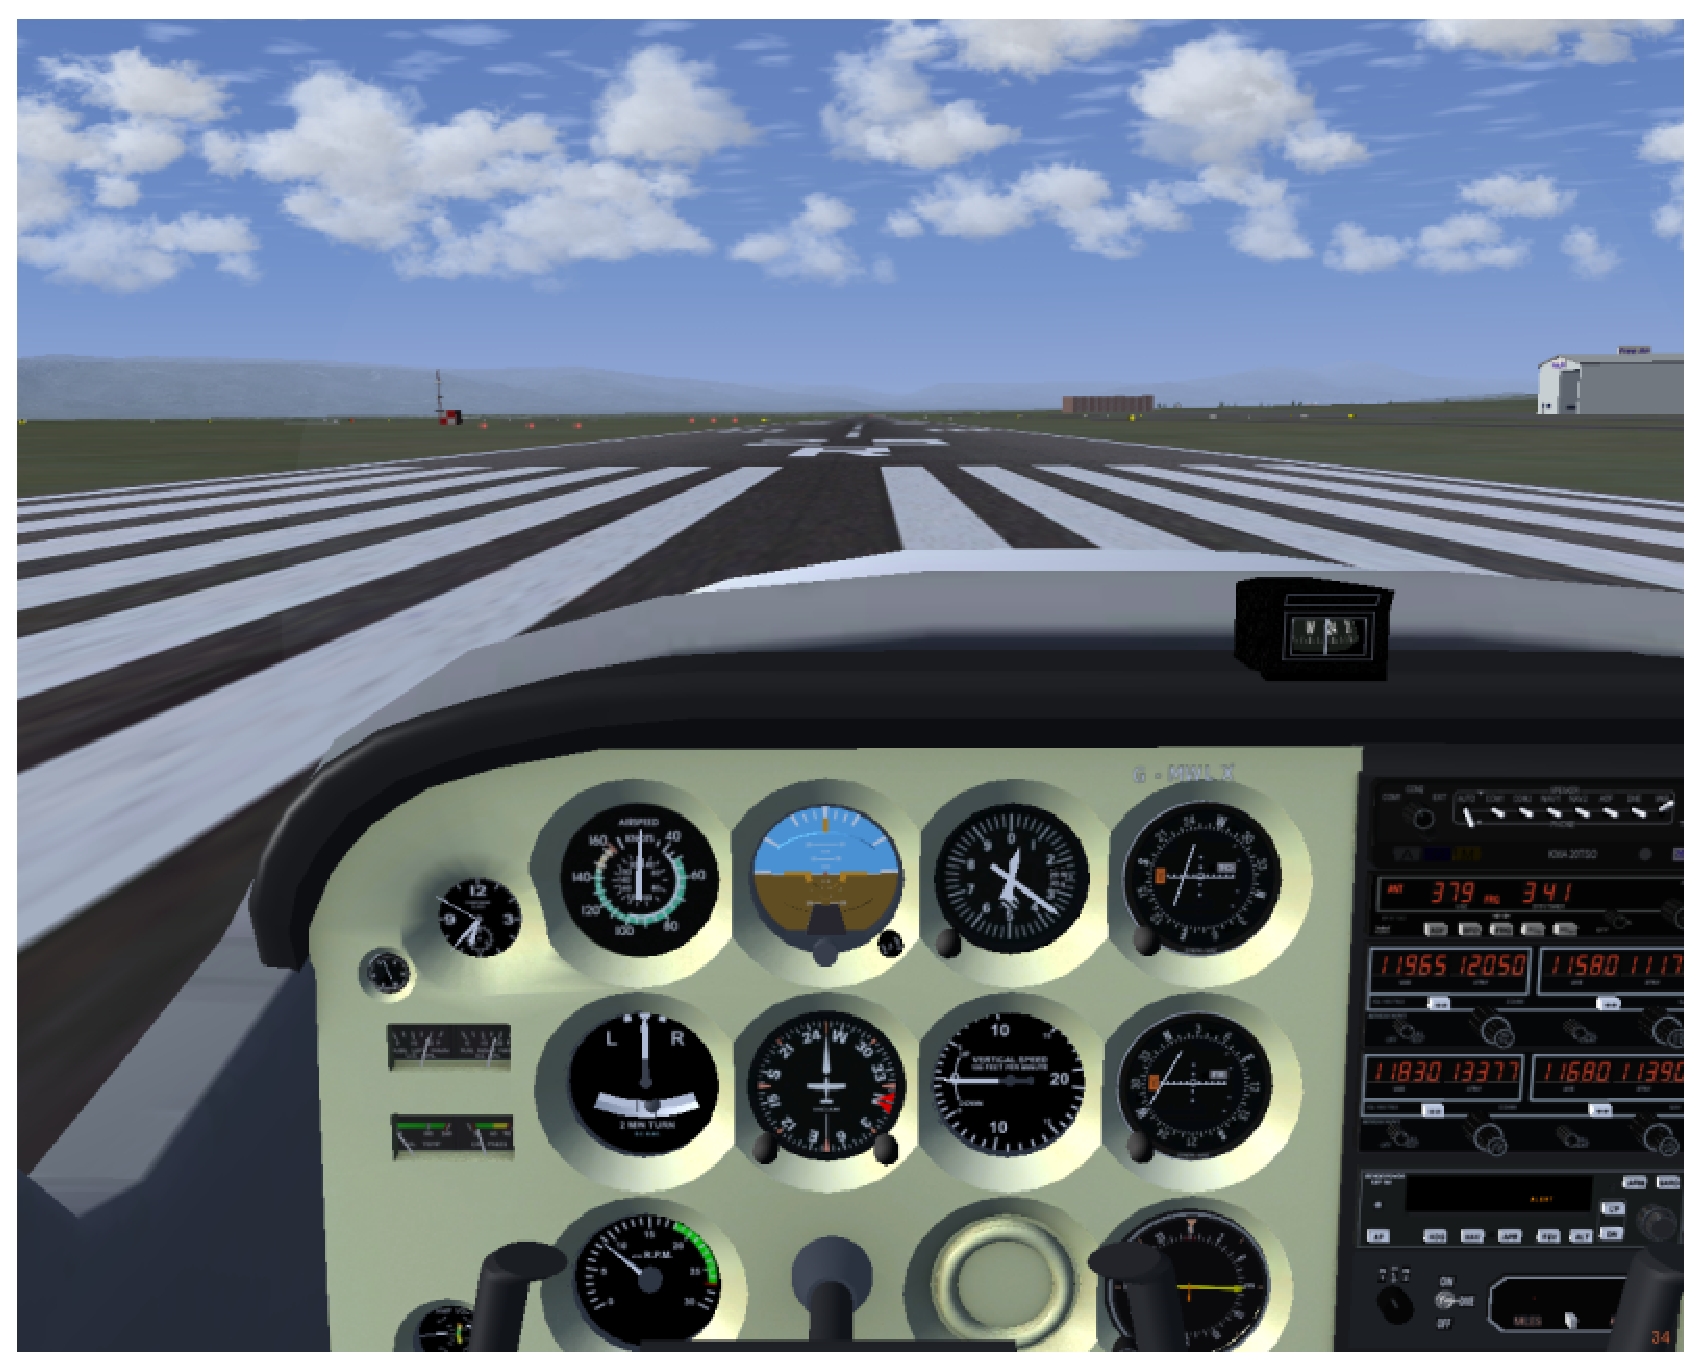
\includegraphics[clip,width=12.5cm]{panel3d}
}}

\smallskip
 \noindent
Fig.\,6: \textit{The 3D cockpit of the Cessna 172.}
\medskip

Aircraft within \FlightGear{} can have both a 2-dimensional instrument panel
and a 3-dimensional cockpit. The 3-dimensional cockpit provide a much
more realistic pilot-eye view, but can be difficult to read with small
monitors.

The default Cessna 172P (c172p) has both a 3-dimensional and 2-dimensional
cockpit. The 3-dimensional cockpit is actived by default when you start
\FlightGear{}, but you can over-lay the 2-dimensional instrument panel by
selecting View -> Toggle 2D Panel from the menu, or pressing the ``P'' key.

While a complete description of all the functions of the instrument panel
of a Cessna is beyond the scope of this guide, we will at least try to outline
the main \Index{flight instrument}s or \Index{gauge}s.

All panel levers and knobs can be operated with the mouse To change a
control, just click with the left/middle mouse button on the
corresponding knob/lever.

Let us start with the most important instruments any simulator pilot must know.
In the
center of the instrument panel (Fig.\,5), in the upper row, you will find the
\Index{artificial horizon} (\Index{attitude indicator}) displaying \Index{pitch}
and
\Index{bank} of your plane. It has pitch marks as well as bank marks at 10, 20,
30, 60,
and 90 degrees.

Left to the artificial horizon, you'll see the \Index{airspeed indicator}. Not
only does
it provide a speed indication in knots but also several arcs showing
characteristic
\Index{velocity rages} you have to consider. At first, there is a green arc
indicating
the normal operating range of speed with the \Index{flaps} fully retracted. The
white arc
indicates the range of speed with flaps in action. The yellow arc shows a range,
which
should only be used in smooth air. The upper end of it has a red radial
indicating the
speed you must never exceeded - at least as long as you won't brake your plane.

Below the airspeed indicator you can find the \Index{turn indicator}. The
airplane in the
middle indicates the roll of your plane. If the left or right wing of the plane
is
aligned with one of the marks, this would indicate a standard turn, i.e\. a turn
of 360
degrees in exactly two minutes.

Below the plane, still in the turn indicator, is the \Index{inclinometer}. It
indicates
if \Index{rudder} and \Index{aileron}s are coordinated. During turns, you always
have to
operate \Index{aileron} and \Index{rudder} in such a way that the ball in the
tube
remains centered; otherwise the plane is skidding. A simple rule says:
``Step onto the ball'', i.e\. step onto the left rudder pedal in case
the ball is on the l.h.s.
\medskip

If you don't have pedals or lack the experience to handle the proper
ratio between aileron/rudder automatically, you can start \FlightGear{}
with the option \texttt{-$ $-enable-auto-coordination}.\index{auto
coordination}

To the r.h.s of the artificial horizon you will find the \Index{altimeter}
showing the height
above sea level (not ground!) in hundreds of feet.  Below the altimeter is the
\Index{vertical speed indicator} indicating the rate of climbing or sinking of
your plane
in hundreds of feet per minute. While you may find it more convenient to use
then the
altimeter in cases, keep in mind that its display usually has a certain lag in
time.

Further below the vertical speed indicator is the RPM (rotations per minute)
indicator\index{RPM indicator}, which displays the rotations per minute  in 100
RPMs. The
green arc marks the optimum region for long-time flight.

The group of the main instruments further includes the \Index{gyro compass}
being
situated below the artificial horizon. Besides this one, there is a
\Index{magnetic
compass} sitting on top of the panel.

Four of these gauges being arranged in the from of a ``T'' are of special
importance: The
air speed indicator, the artificial horizon, the altimeter, and the compass
should be
scanned regularly during flight.

Besides these, there are several supplementary instruments. To the very
left you will find the \Index{clock}, obviously being an important tool
for instance for determining turn rates.Below the clock there are
several smaller gauges displaying the technical state of your engine.
Certainly the most important of them is the \Index{fuel indicator} - as
any pilot should know.

The \Index{ignition switch} is situated in the lower left corner of the
panel (cf. Fig.\,4). It has five positions: ``OFF'', ``L'', ``R'',
``BOTH'', and ``START''. The first one is obvious. ``L'' and ``R'' do
not refer to two engines (actually the Cessna does only have one) but
to two magnetos being present for safety purposes. The two switch
positions can be used for test puposes during preflight. During normal
flight the switch should point on ``BOTH''. The extreme right position
is for \index{starting the engine} using a battery-powered
\Index{starter} (to be operated with the ``s'' key in flight gear).

Like in most flight simulators, you actually get a bit more than in a
real plane. The red field directly below the gyro compass displays the
state of the \Index{brakes}, i.e., it is lit in case of the brakes
being engaged. The instruments below indicate the position of
your\Index{yoke}. This serves as kind of a compensation for the missing
forces you feel while pushing a real \Index{yoke}. Three of the arrows
correspond to the three axes of your yoke/pedal controlling nose
up/down, bank left/right, rudder left/right, and throttle. (Keep in
mind: They do \textbf{not} reflect the actual position of the plane!)
The left vertical arrow indicates elevator trim.

The right hand side of the panel is occupied by the \Index{radio stack}. Here
you find
two \Index{VOR} receivers (NAV),\index{NAV} an \Index{NDB} receiver
(\Index{ADF}) and two \Index{communication radio}s
(COMM1/2)\index{COMM1}\index{COMM2} as
well as the autopilot.

The \Index{communication radio} is used for communication with \Index{air
traffic
facilities}; it is just a usual radio transceiver working in a special frequency
range.
The frequency is displayed in the ``COMM'' field. Usually there are two
\Index{COM
transceiver}s; this way you can dial in the frequency of the next controller to
contact
while still being in contact with the previous one.

The COM radio can be used to display \Index{ATIS} messages as well. For
this purpose, just to dial in the ATIS frequency of the relevant
airport.

The \Index{VOR} (Very High Frequency Omni-Directional Range) receiver is used
for course
guidance during flight. The frequency of the sender is displayed in the
''\Index{NAV}'' field. In a sense,
a VOR acts similarly to a light house permitting to display the position of the
aircraft on a radial around the sender. It transmits one omni-directional ray of
radio
waves plus a second ray, the phase of which differs from the first one depending
on its
direction (which may be envisaged as kind of a ``rotating'' signal). The phase
difference between the two
signals allows evaluating the angle of the aircraft on a 360 degrees circle
around the VOR sender, the so-called radial. This radial is then displayed on
the gauges
NAV1 and NAV2, resp., left to frequency field. This way it should be clear that
the VOR display, while
indicating the position of the aircraft relative to the VOR sender, does not say
anything about the orientation of the plane.

Below the two COM/NAV devices is an \Index{NDB} receiver called ADF (automatic
direction
finder). Again there is a field displaying the frequency of the facility. The
ADF can be
used for navigation, too, but contrary to the VOR does not show the position of
the plane
in a radial relative to the sender but the direct heading from the aircraft to
the
sender. This is displayed on the gauge below the two NAV gauges.

Above the COMM1 display you will see three LEDs in the colors blue, amber, and
white
indicating the outer, middle, and, inner, resp\. marker beacon.\index{marker,
outer}\index{marker, inner}\index{marker, middle} These show the distance to the
runway
threshold during landing. They do not require the input of a frequency.

Below the radios you will find the \Index{autopilot}. It has five keys
for WL = ``Wing-Leveler'', ``HDG'' = ``Heading'', NAV, APR =
``Glide-Slope'', and ALT = ``Altitude''. These keys when engaged hold
the corresponding property.

You can change the numbers for the radios using the mouse. For this
purpose, click left/right to the circular knob below the corresponding
number. The corresponding switch left to this knob can be used for
toggling between the active/standby frequency.

A detailed description of the workings of these instruments and their use for
navigation
lies beyond this Guide; if you are interested in this exciting topic, we suggest
consulting a book on instrument flight (simulation). Besides, this would be
material for
a yet to be written \FlightGear{} Flight School.

It should be noted, that you can neglect these radio instruments as
long as you are strictly flying according to \Index{VFR} (\Index{visual
flight rules}). For those wanting to do \Index{IFR} (\Index{instrument
flight rules}) flights, it should be mentioned that \FlightGear{}
includes a huge database of \Index{navaids} worldwide.

Finally, you find the \Index{throttle}, \Index{mixture}, and flap
control\index{flaps} in
the lower right of the panel (recall, flaps can be set via $[$ and $]$ or just
using the mouse).

As with the keyboard, the panel\index{panel!reconfiguration} can be
re-configured using
configuration files. As these have to be plane specific, they can be found under
the
directory of the corresponding plane. As an example, the configuration file for
the
default Cessna C172 can be found at \texttt{FlightGear/Aircraft/c172/Panels} as
\texttt{c172-panel.xml}. The accompanying documentation for customizing it
(i.e\. shifting,
replacing etc\. gauges and more) is contained in the file
\texttt{README.xmlpanel}\index{README.xmlpanel}
written by John Check\index{Check, John},
to be found in the source code in the directory \texttt{docs-mini}.

\medskip

\centerline{\fbox{
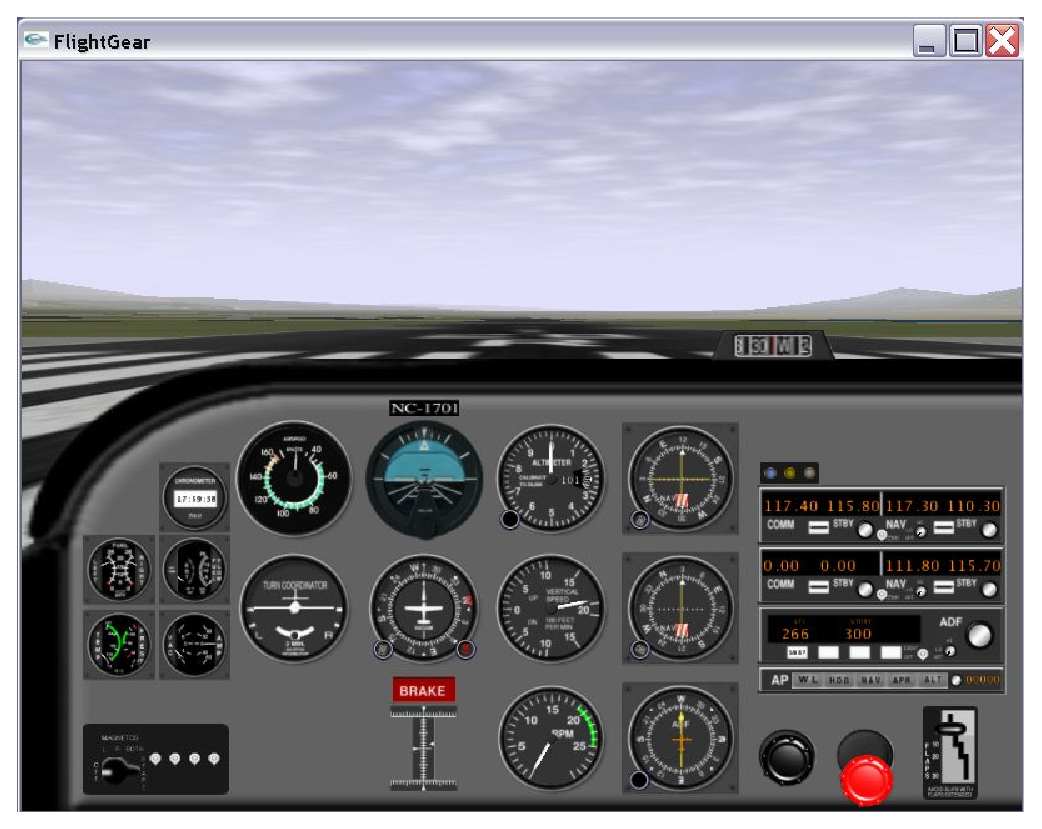
\includegraphics[clip,width=12.5cm]{panel5}
}}

\smallskip
 \noindent
Fig.\,5: \textit{The Cessna 172p 2-D instrument panel.}
\medskip

%%%%%%%%%%%%%%%%%%%%%%%%%%%%%%%%%%%%%%%%%%%%%%%%%%%%%%%%%%%%%%%%%%%%%%%%%%%%%%%%
%%%%%%%%%%%%%%%
\section{The Head Up Display\index{head up display}}
%%%%%%%%%%%%%%%%%%%%%%%%%%%%%%%%%%%%%%%%%%%%%%%%%%%%%%%%%%%%%%%%%%%%%%%%%%%%%%%%
%%%%%%%%%%%%%%%

At current, there are two options for reading off the main flight parameters of
the
plane: One is the instrument panel already mentioned, while the other one is the
\Index{HUD} (\textbf{H}ead \textbf{U}p \textbf{D}isplay) \index{head up
display}. Neither
are \Index{HUD}s used in usual general aviation planes nor in civilian ones.
Rather they
belong to the equipment of modern military jets. However, some might find it
easier to
fly using the HUD even with general aviation aircraft. Several \Index{Cessna}
pilots
might actually love to have one, but technology is simply too expensive for
implementing
HUDs in general aviation aircraft. Besides, the HUD displays several useful
figures
characterizing simulator performance, not to be read off from the panel.

The \Index{HUD} shown in Fig.\,7  displays all main flight parameters of the
plane. In
the center you find the \Index{pitch indicator} (in degrees) with the
\Index{aileron
indicator} above and the \Index{rudder indicator} below. A corresponding scale
for the
elevation\index{elevation indicator} can be found to the left of the pitch
scale. On the
bottom there is a simple \Index{turn indicator}.

There are two scales at the extreme left: The inner one displays the
\Index{speed} (in
kts) while the outer one indicates position of the \Index{throttle}. The Cessna
172 takes
off at around 55 kts. The two scales on the extreme r.h.s display your
\Index{height},
i.\,e\. the left one shows the height above ground while the right of it gives
that above
zero, both being displayed in feet.

Besides this, the \Index{HUD} delivers some additions information. On the upper
left you
will find date and time. Besides,  \Index{latitude} and \Index{longitude},
resp., of your current position are shown on top.

You can change color of the \textbf{HUD} using the ``H'' or ``'h''  key.
Pressing the toggle ``i/I'' minimizes/maximizes the HUD.

\medskip

 \centerline{\fbox{
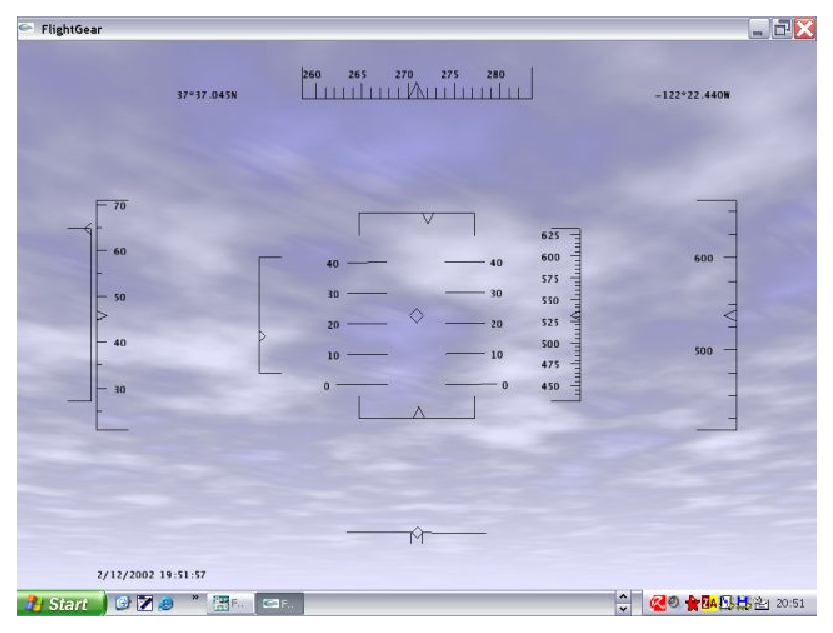
\includegraphics[clip,width=12.5cm]{hud2}
}}

\smallskip
 \noindent
Fig.\,7: \textit{The HUD, or Head Up Display.}
\medskip

%%%%%%%%%%%%%%%%%%%%%%%%%%%%%%%%%%%%%%%%%%%%%%%%%%%%%%%%%%%%%%%%%%%%%%%%%%%%%%%%
%%%%%%%%%%%%%%%
\section{Mouse controlled actions\index{mouse, actions}}
%%%%%%%%%%%%%%%%%%%%%%%%%%%%%%%%%%%%%%%%%%%%%%%%%%%%%%%%%%%%%%%%%%%%%%%%%%%%%%%%
%%%%%%%%%%%%%%%

Besides just clicking the menues, your mouse has got certain valuable functions
in \FlightGear{}.


There are three \Index{mouse modes}.\index{mouse} In the normal mode
(pointer cursor) panel's controls can be operated with the mouse. To
change a control, click with the left/middle mouse button on the
corresponding knob/lever. While the left mouse button leads to small
increments/decrements, the middle one makes greater ones. Clicking on
the left hand side of the knob/lever decreases the value, while
clicking on the right hand side increases it.

 Right clicking the mouse activates the simulator control mode (cross
 hair cursor). This allows control of aileron/elevator via the mouse in
 absence of a joystick/yoke (enable \texttt{-$
 $-enable-auto-coordination} in this case). If you have a joystick you
 certainly will not make use of this mode

 Right clicking the mouse another time activates the view control mode (arrow
cursor).
 This allows changing direction of view, i.e. pan and tilt the view, via the
mouse.
 Clicking the left mouse button resets the view.
 Dragging using the middle mouse button moves the viewpoint itself.

 Right clicking the mouse once more resets it into the initial state.

If you are looking for some interesting \Index{places to discover} with
\FlightGear{}
(which may or may not require downloading additional scenery) you may want to
check
 \medskip

 \web{http://www.flightgear.org/Places/}.
  \medskip

\noindent
 There is now a menu entry for entering directly the \Index{airport code} of the
airport you want to start from.

Finally, if you're done and are about to leave the plane, just hit the ESC key
or use the
corresponding menu entry to \Index{exit} the program. It is not suggested that
you simply
``kill'' the simulator using Ctrl-C on the text window.



%% Revision 0.00  1998/09/08  michael
%% Initial revision for version 0.53.
%% Revision 0.01  1998/09/20  michael
%% several extensions and corrections, added Fig.1.
%% revision 0.10  1998/10/01  michael
%% final proofreading for release
%% revision 0.11  1998/11/01  michael
%% Complete revision of keyborad controls, interesting places
%% revision 0.12  1999/03/07  michael
%% Corrected rudder key
%% revision 0.20  1999/06/04  michael
%% HUD completely rewritten, added panel section with picture, and menu section
%% updated keystrokes
%% revision 0.3 2000/04/20 michael
%% again updated and added keystrokes
%% revised menu entries
%% picture of new panel and re-written panel section
%% added mouse control section
%% Updated many keys, notably autopilot related, added two new tables
%% revision 0.4 2001/05/12 michael
%% updated/added many keystrikes, updated/added panel description
%% (radio stack etc.), new panel pic, panel before HUD now
%% short description of VOR/NDB
%% revision 0.41 2001/01/01 michael
%% added section on flight school material
%% added hints to user configurable *.xml files
%% revision 0.5 2002/01/01 michael
%% revised all changed keybindings now mostly read off of keyboard.xml
%% restructured tables more logically and put into separate files
%% for inclusion in Short Reference
%% New panel picture and revised descirption of panel according to new features
%% New HUD picture
%% revision 0.6 2002/09/05 michael
%% Several corrections/tweaks in plus renumbering of tables
%% Tweaks in menu entries
%% Added 3D cockpit picture
%% Changing numbers in radios
%% Added new menu items, swapped over 3D and 2-D pictures, as 3D cockpit is
%%  now the default
